\section{Choix des cellules}
Les cellules sont la clef de voute de notre simulation, étant donné qu'elles sont les éléments principaux de celle-ci. 
La première difficulté à été de trouver quel type de cellule nous allions étudier. Pour cela nous avons effectué certaines recherches, pour trouver des cellules simples à comprendre, à manipuler et à représenter.
Cela impliquait différents facteurs : 
\begin{description}
  \item[La taille des cellules] : les bactéries sont environ 10 fois plus petites que les cellules eucaryotes 
  \item[La durée de division] : élément essentiel pour le programme, et qui varie beaucoup selon les espèces : de 20 minutes à 24h, respectivement pour les bactéries et les cellules humaines
  \item[Le métabolisme] : les éléments nutritionnels, le fait de survivre en aérobie ou non, et autre facteurs environnementaux
  \item[Le déplacement des cellules] : il existe tout types de cellules qui se déplacent ou non, et de différentes manières
  \item[L'organisation] : cellules isolées, colonies, ou organismes multi-cellulaires
\end{description}

\begin{figure}[H]
	\centering
	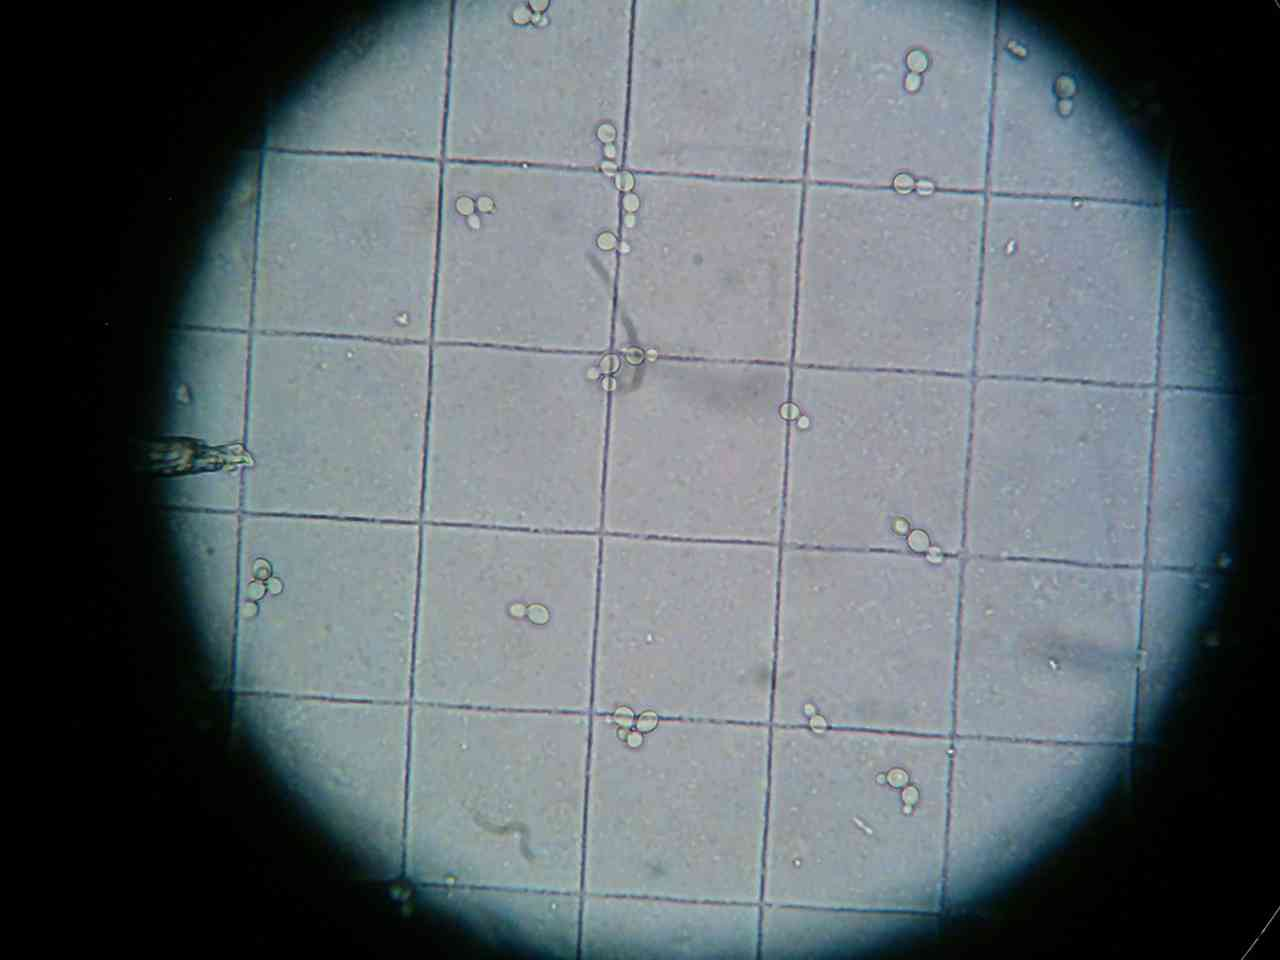
\includegraphics[width=15em]{Images/malassez.JPG}
	\caption{Cellules de Malassez}
\end{figure}

Initialement nous n'étions pas fixés sur le choix d'un type de cellule en particulier, il en découle que le programme, qui avait commencé à être développé en parallèle, peut être configuré pour certains des facteurs.

Ainsi nous avons choisi les levures, qui sont des organismes unicellulaires qui forment des colonies, qui on fait l'objet de nombreuses études précédentes. Ce qui nous a permis d'accéder facilement à des informations les concernant.
De plus les levures sont facilement mises en culture ce qui nous a permis de faire de nous en procurer facilement et de faire nos propres expériences. 

\section{Expérience personnelle}
Nous avons fait cette expérience pour avoir une idée de l'effet des UV sur les colonies de levures. 
Notre but était de soumettre les colonies à différents temps d'exposition\footnote{Mais à puissance constante}. 
Nous avions pour projet l'observation au microscope des colonies afin de dénombrer les clones mutés et le 
taux de mortalité en fonction de la durée d'exposition.
Nous voulions procéder à l'aide de lame de comptage telles que les «~cellules de Malassez~»\ref{SitoMala}.

Pour cela nous avons eu besoin de l'aide de notre professeur référent en Sciences de la Vie et de la Terre.
Ainsi à l'aide de Madame Sirlin et de X\footnote{assistante ?}, nous avons réalisé cette expérience, selon le protocole définit ci-après.

\subsection{Protocole}
  \subsubsection{Matériel}
    \begin{itemize}
      \item Six boites de pétri
      \item Des marqueurs
      \item De la levure
      \item Deux lampes à alcool
      \item Une pipette râteau
      \item De la verrerie : bécher, tube à essai …
    \end{itemize}
  \subsubsection{Étapes}
    Tout d'abord il faut créer la gélose dans laquelle nous avons ajouté du glucose, afin de constituer un environnement riche pour le développement des levures. La gélose est une substance composée d'agar-agar, sur laquelle nous allons ensemencer les souches de levure.
    
    Nous avons parallèlement produit une solution de levure de boulanger à faible concentration. 
    
    Nous avons répandu la gélose dans les boites de pétri et attendu qu'elle se solidifie. Puis, à l'aide d'une d'une pipette râteau, dans un environnement stérilisé par les lampes à alcool, nous avons répandu la solution de levure et d'eau chaude sur le milieu. 
    
    Nous avons crée 6 cultures : 
    \begin{itemize}
      \item Deux témoins qui ne seraient pas exposés aux UV
      \item Deux test qui seraient exposés aux UV durant une nuit
      \item Deux autres test qui seraient exposés aux UV durant 24h
    \end{itemize}
    
    \begin{figure}[H]
			\begin{center}
				\includegraphics[width=20em]{Images/six_levures.JPG}
				\includegraphics[width=20em]{Images/levure.JPG}
			\end{center}
			\caption{Les six boites de pétri}
		\end{figure}

\subsection{Interprétation et résultats}
  Inopportunément, nous n'avons pas eu accès à des microscopes pour analyser les résultats. De plus nous avions utilisé de la levure de boulanger, alors que pour observer des mutations visibles, il aurait fallu des levures ADE2. Malgré tout nous avons bien constaté à l'œil nu la grande disparité du nombre de colonies entre les différents test et témoins. Et donc, n'avons pu que constater la mortalité des UV, mais nous n'avons pas pu calculer des taux précis.
  Ce genre d'expérience est courante et nous avons pu trouver des résultats probants aussi bien que dans les livres de seconde et première\footnote{\ref{BibSito}}, et des expériences similaires sur internet. Ce qui nous a permis d'enchaîner facilement sur la réalisation du programme.

\subsection{Recherches complémentaires}
  Grâce à plusieurs sources nous avons obtenus les informations nécessaires au programme que nous n’avions pas pu récupérer avec l’expérience. Nos sources principales sont : le livre de première de SVT chapitre sur la génétique, activité sur l’exposition de levures aux UV et un site internet d’un professeur de SVT qui proposé le protocole et le résultat de cette même expérience\footnote{Cf \ref{BibSito}}. Dans chacun des cas nous avons pu obtenir le tableau récapitulatif des morts et mutation des levures en fonction du temps. C’est ces données que nous avons pu implémenter dans ce programme pour rendre la simulation plus ou moins réaliste lors de l’utilisation de la « fonction UV ». De plus le protocole trouvé sur internet a pu nous donner une idée de comment nous allions procéder lors de notre propre expérience. Enfin ces données ont vraiment pu compléter celles déduites de notre expérience qui, après coup, n’a pu nous fournir les informations voulues.
  
  C'est ainsi que nous avons trouvé que les levures, comme les cellules humaines, avaient un vieillissement cellulaires qui les prédéterminaient à une mort certaine environ après leur 50ème division\footnote{Cf \ref{BibSito}}
  
\subsection{Conclusion}
  À partir des informations recherchées et des interprétations que nous en avons faites, nous avons pu nous lancer dans la véritable réalisation du projet de simulation.
